\documentclass[lesson_slides]{subfiles}
%\usepackage{natbib}
\usepackage{graphicx}
% \graphicspath{ {./images/} }
\usepackage{enumerate}
\usepackage{pifont} % for ding
\usepackage{float} % keeps tables in the exact position they occupy in the code
\usepackage{xcolor} % text colour
\usepackage{gb4e} % leave last

\begin{document}
%%=-=-=-=-=-=-=-=-=-=-=-=-=-=-=-=-=-=-=-=-=-=-=-=-=-=-=-=-=-=-=-=-=-=-=-=-=-=-=-=
%   FRAME START   -=-=-=-=-=-=-=-=-=-=-=-=-=-=-=-=-=-=-=-=-=-=-=-=-=-=-=-=-=-=-=
\begin{frame}[c]{Discussion}

\begin{center}
    \textbf{What does the data mean in our theory?}
\end{center}
  
\end{frame}
%   FRAME END   --==-=-=-=-=-=-=-=-=-=-=-=-=-=-=-=-=-=-=-=-=-=-=-=-=-=-=-=-=-=-=
%   FRAME START   -=-=-=-=-=-=-=-=-=-=-=-=-=-=-=-=-=-=-=-=-=-=-=-=-=-=-=-=-=-=-=
\begin{frame}[c]{Discussion}
    
\begin{center}
    \textbf{First change}
\end{center}
  
\end{frame}
%   FRAME END   --==-=-=-=-=-=-=-=-=-=-=-=-=-=-=-=-=-=-=-=-=-=-=-=-=-=-=-=-=-=-=
%   FRAME START   -=-=-=-=-=-=-=-=-=-=-=-=-=-=-=-=-=-=-=-=-=-=-=-=-=-=-=-=-=-=-=
\begin{frame}[c]{From predominant wh-ex situ to predominant wh-in situ}

\begin{columns}
    \column{0.5\textwidth}
        \centering
        \textbf{\textsc{the decline of wh-ex situ}}
    \begin{center}
        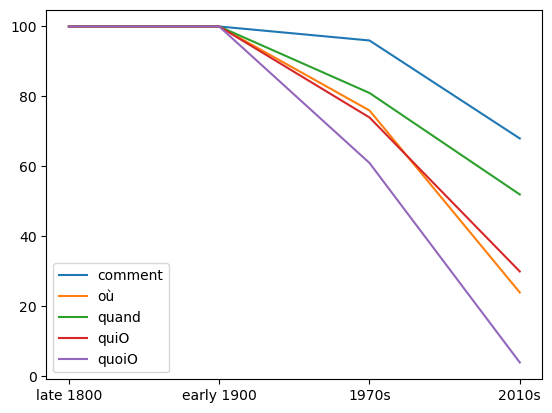
\includegraphics[width=\linewidth]{images/all.png}
    \end{center}
    \column{0.5\textwidth}
        \centering
        \textbf{\textsc{the rise of wh-in situ}}
        \begin{center}
        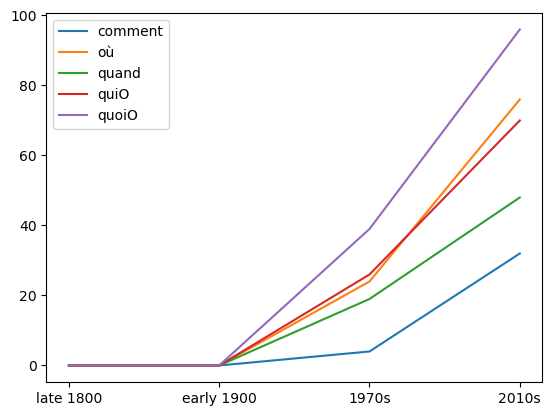
\includegraphics[width=\linewidth]{images/insitu.png}
    \end{center}
    \end{columns}
  
\end{frame}
%   FRAME END   --==-=-=-=-=-=-=-=-=-=-=-=-=-=-=-=-=-=-=-=-=-=-=-=-=-=-=-=-=-=-=

%   FRAME START   -=-=-=-=-=-=-=-=-=-=-=-=-=-=-=-=-=-=-=-=-=-=-=-=-=-=-=-=-=-=-=
\begin{frame}[c]{From predominant wh-ex situ to predominant wh-in situ}

        \transboxin<1>
        \transglitter<2>
        % \transwipe<3>
        \textbf{\textsc{french has evolved in the direction of predominant im$=$0}} \pause

        \begin{table}[H]
        \centering
        \begin{tabular}{|l|r|r|r|r|}
        \hline
         & Merge & Spell Out & IM & IM\textsubscript{lex} \\
        \hline
        late 1800 & 1 & n/a & 0 & n/a \\
        \hline
        early 1900 & 1 & n/a & 0 & n/a \\
        \hline
        1970s & 1 & n/a & 0/1 & n/a \\
        \hline
        2010s & 1 & n/a & 0/1 & n/a \\
        \hline
        \end{tabular}
        \caption{\label{tab:samp}Parametric settings for the French FocusP: evolution over time.}
    \end{table}
  
\end{frame}
%   FRAME END   --==-=-=-=-=-=-=-=-=-=-=-=-=-=-=-=-=-=-=-=-=-=-=-=-=-=-=-=-=-=-=
%   FRAME START   -=-=-=-=-=-=-=-=-=-=-=-=-=-=-=-=-=-=-=-=-=-=-=-=-=-=-=-=-=-=-=
\begin{frame}[c]{From predominant wh-ex situ to predominant wh-in situ}

        \textbf{\textsc{french has evolved in the direction of predominant im$=$0}}

        \begin{table}[H]
        \centering
        \begin{tabular}{|l|r|r|r|r|}
        \hline
         & Merge & Spell Out & IM & IM\textsubscript{lex} \\
        \hline
        late 1800 & 1 & n/a & \textcolor{red}{0} & n/a \\
        \hline
        early 1900 & 1 & n/a & \textcolor{red}{0} & n/a \\
        \hline
        1970s & 1 & n/a & 0/1 & n/a \\
        \hline
        2010s & 1 & n/a & 0/1 & n/a \\
        \hline
        \end{tabular}
        \caption{\label{tab:samp}Parametric settings for the French FocusP: evolution over time.}
    \end{table}
  
\end{frame}
%   FRAME END   --==-=-=-=-=-=-=-=-=-=-=-=-=-=-=-=-=-=-=-=-=-=-=-=-=-=-=-=-=-=-=
%   FRAME START   -=-=-=-=-=-=-=-=-=-=-=-=-=-=-=-=-=-=-=-=-=-=-=-=-=-=-=-=-=-=-=
\begin{frame}[c]{From predominant wh-ex situ to predominant wh-in situ}

        \textbf{\textsc{french has evolved in the direction of predominant im$=$0}}

        \begin{table}[H]
        \centering
        \begin{tabular}{|l|r|r|r|r|}
        \hline
         & Merge & Spell Out & IM & IM\textsubscript{lex} \\
        \hline
        late 1800 & 1 & n/a & \textcolor{red}{0} & n/a \\
        \hline
        early 1900 & 1 & n/a & \textcolor{red}{0} & n/a \\
        \hline
        1970s & 1 & n/a & \hl{0/1} & n/a \\
        \hline
        2010s & 1 & n/a & \hl{0/1} & n/a \\
        \hline
        \end{tabular}
        \caption{\label{tab:samp}Parametric settings for the French FocusP: evolution over time.}
    \end{table}
  
\end{frame}
%   FRAME END   --==-=-=-=-=-=-=-=-=-=-=-=-=-=-=-=-=-=-=-=-=-=-=-=-=-=-=-=-=-=-=
%   FRAME START   -=-=-=-=-=-=-=-=-=-=-=-=-=-=-=-=-=-=-=-=-=-=-=-=-=-=-=-=-=-=-=
\begin{frame}[c]{From predominant wh-ex situ to predominant wh-in situ}

        \textbf{\textsc{french has evolved in the direction of predominant im$=$0}}

        \begin{table}[H]
        \centering
        \begin{tabular}{|l|r|r|r|r|}
        \hline
         & Merge & Spell Out & IM & IM\textsubscript{lex} \\
        \hline
        late 1800 & 1 & n/a & \textcolor{red}{0} & n/a \\
        \hline
        early 1900 & 1 & n/a & \textcolor{red}{0} & n/a \\
        \hline
        1970s & 1 & n/a & \hl{0 (22\%) /1 (78\%)} & n/a \\
        \hline
        2010s & 1 & n/a & \hl{0/1} & n/a \\
        \hline
        \end{tabular}
        \caption{\label{tab:samp}Parametric settings for the French FocusP: evolution over time.}
    \end{table}
  
\end{frame}
%   FRAME END   --==-=-=-=-=-=-=-=-=-=-=-=-=-=-=-=-=-=-=-=-=-=-=-=-=-=-=-=-=-=-=
%   FRAME START   -=-=-=-=-=-=-=-=-=-=-=-=-=-=-=-=-=-=-=-=-=-=-=-=-=-=-=-=-=-=-=
\begin{frame}[c]{From predominant wh-ex situ to predominant wh-in situ}

        \textbf{\textsc{french has evolved in the direction of predominant im$=$0}}

        \begin{table}[H]
        \centering
        \begin{tabular}{|l|r|r|r|r|}
        \hline
         & Merge & Spell Out & IM & IM\textsubscript{lex} \\
        \hline
        late 1800 & 1 & n/a & \textcolor{red}{0} & n/a \\
        \hline
        early 1900 & 1 & n/a & \textcolor{red}{0} & n/a \\
        \hline
        1970s & 1 & n/a & \hl{0 (22\%) / 1 (78\%)} & n/a \\
        \hline
        2010s & 1 & n/a & \hl{0 (64\%) / 1 (36\%)} & n/a \\
        \hline
        \end{tabular}
        \caption{\label{tab:samp}Parametric settings for the French FocusP: evolution over time.}
    \end{table}
  
\end{frame}
%   FRAME END   --==-=-=-=-=-=-=-=-=-=-=-=-=-=-=-=-=-=-=-=-=-=-=-=-=-=-=-=-=-=-=
%   FRAME START   -=-=-=-=-=-=-=-=-=-=-=-=-=-=-=-=-=-=-=-=-=-=-=-=-=-=-=-=-=-=-=
\begin{frame}[c]{From predominant wh-ex situ to predominant wh-in situ}


    \transboxin<1>
    \transglitter<2>
    \transwipe<3>
    \noindent \textbf{\textsc{our understanding of french interrogative wh-movement}} \pause
    \begin{enumerate}
        \item French was a wh-fronting language (IM$=$0 for FocusP) up until at least the beginning of the 20\textsuperscript{th} century;\pause
        \item French has been characterized by movement optionality (IM$=$0/1) since at least the beginning of the 1970s; \pause
        \item French has moved in the direction of a near-generalisation of the in situ strategy between 1970 and 2014; \pause 
        \item French will evolve to either: \pause
        \begin{itemize}
            \item lose wh-fronting altogether (IM=0); \pause
            \item develop a specialised meaning for each strategy (cf. \cite{faure2021exclusivity}).
        \end{itemize}    
    \end{enumerate}
  
\end{frame}
%   FRAME END   --==-=-=-=-=-=-=-=-=-=-=-=-=-=-=-=-=-=-=-=-=-=-=-=-=-=-=-=-=-=-=
%   FRAME START   -=-=-=-=-=-=-=-=-=-=-=-=-=-=-=-=-=-=-=-=-=-=-=-=-=-=-=-=-=-=-=
\begin{frame}[c]{Discussion}
    
\begin{center}
    \textbf{Second change}
\end{center}
  
\end{frame}
%   FRAME END   --==-=-=-=-=-=-=-=-=-=-=-=-=-=-=-=-=-=-=-=-=-=-=-=-=-=-=-=-=-=-=

%   FRAME START   -=-=-=-=-=-=-=-=-=-=-=-=-=-=-=-=-=-=-=-=-=-=-=-=-=-=-=-=-=-=-=
\begin{frame}[c]{Towards predominant no head-movement/activation}

    \textbf{\textsc{the decline of vs and rise of sv}}
    \begin{center}
        \includegraphics[width=10cm, height=6cm]{images/exsituinsitu.png}
    \end{center}
  
\end{frame}
%   FRAME END   --==-=-=-=-=-=-=-=-=-=-=-=-=-=-=-=-=-=-=-=-=-=-=-=-=-=-=-=-=-=-=
%   FRAME START   -=-=-=-=-=-=-=-=-=-=-=-=-=-=-=-=-=-=-=-=-=-=-=-=-=-=-=-=-=-=-=
\begin{frame}[c]{Towards predominant no head-movement/activation}

    \transboxin<1>
    \transglitter<2>
    %\transwipe<3>
    \textbf{\textsc{french has evolved in the direction of im\textsubscript{lex}$=$0 and spellout$=$0}} \pause

    \noindent Up until at least the 1930s, French required spelling out the head of Focus (SpellOut=1, see \cite{roberts2017} for an understanding of French enclitics as an inflectional class) and merging the finite verb (IM\textsubscript{lex}) almost systematically. \pause

    \begin{table}[H]
        \centering
        \begin{tabular}{|r|r|r|r|r|r|}
        \hline
        Merge & Spell Out & IM  & IM\textsubscript{lex} \\
        \hline
        1 & 1 & 0 & 1 \\
        \hline
        \end{tabular}
        \caption{\label{tab:samp}Parametric settings for the French FocusP: VS.}
    \end{table}
  
\end{frame}
%   FRAME END   --==-=-=-=-=-=-=-=-=-=-=-=-=-=-=-=-=-=-=-=-=-=-=-=-=-=-=-=-=-=-=
%   FRAME START   -=-=-=-=-=-=-=-=-=-=-=-=-=-=-=-=-=-=-=-=-=-=-=-=-=-=-=-=-=-=-=
\begin{frame}[c]{Towards predominant no head-movement/activation}

    \textbf{\textsc{french has evolved in the direction of im\textsubscript{lex}$=$0 and spellout$=$0}}

    \noindent Up until at least the 1930s, French required spelling out the head of Focus (SpellOut=1, see \cite{roberts2017} for an understanding of French enclitics as an inflectional class) and merging the finite verb (IM\textsubscript{lex}) almost systematically.

    \begin{table}[H]
        \centering
        \begin{tabular}{|r|r|r|r|r|r|}
        \hline
        Merge & Spell Out & IM  & IM\textsubscript{lex} \\
        \hline
        1 & \hl{1} & 0 & \hl{1} \\
        \hline
        \end{tabular}
        \caption{\label{tab:samp}Parametric settings for the French FocusP: VS.}
    \end{table}
  
\end{frame}
%   FRAME END   --==-=-=-=-=-=-=-=-=-=-=-=-=-=-=-=-=-=-=-=-=-=-=-=-=-=-=-=-=-=-=
%   FRAME START   -=-=-=-=-=-=-=-=-=-=-=-=-=-=-=-=-=-=-=-=-=-=-=-=-=-=-=-=-=-=-=
\begin{frame}[c]{Towards predominant no head-ovement/activation}

    \transboxin<1>
    \transglitter<2>
    %\transwipe<3>
    \vspace*{-10mm}
    \textbf{\textsc{french has evolved in the direction of im\textsubscript{lex}$=$0 and spellout$=$0}} \pause

\noindent The option of not spelling out Focus^0 (SpellOut=0) existed, but was still rare. This systematically correlates to no movement of the finite verb (IM\textsubscript{lex}=0). \pause

\begin{table}[H]
    \centering
    \begin{tabular}{|r|r|r|r|r|r|}
    \hline
    Merge & Spell Out & IM & IM\textsubscript{lex} \\
    \hline
    1 & 0 & 0 & 0 \\
    \hline
    \end{tabular}
    \caption{\label{tab:samp}Parametric settings for the French FocusP: SV.}
\end{table}
  
\end{frame}
%   FRAME END   --==-=-=-=-=-=-=-=-=-=-=-=-=-=-=-=-=-=-=-=-=-=-=-=-=-=-=-=-=-=-=
%   FRAME START   -=-=-=-=-=-=-=-=-=-=-=-=-=-=-=-=-=-=-=-=-=-=-=-=-=-=-=-=-=-=-=
\begin{frame}[c]{Towards predominant no head-movement/activation}

    \transboxin<1>
    \transglitter<2>
    % \transwipe<3>
    \textbf{\textsc{french has evolved in the direction of im\textsubscript{lex}$=$0 and spellout$=$0}}

\noindent The option of not spelling out Focus^0 (SpellOut$=$0) existed, but was still rare. This systematically correlates to no movement of the finite verb (IM\textsubscript{lex}$=$0).

\begin{table}[H]
    \centering
    \begin{tabular}{|r|r|r|r|r|r|}
    \hline
    Merge & Spell Out & IM & IM\textsubscript{lex} \\
    \hline
    1 & \hl{0} & 0 & \hl{0} \\
    \hline
    \end{tabular}
    \caption{\label{tab:samp}Parametric settings for the French FocusP: SV.}
\end{table}

\noindent The parametrisation in the table above became dominant before the 1970s. \pause

\noindent Forecasted possible evolution: total loss of VS.
  
\end{frame}
%   FRAME END   --==-=-=-=-=-=-=-=-=-=-=-=-=-=-=-=-=-=-=-=-=-=-=-=-=-=-=-=-=-=-=
%   FRAME START   -=-=-=-=-=-=-=-=-=-=-=-=-=-=-=-=-=-=-=-=-=-=-=-=-=-=-=-=-=-=-=
\begin{frame}[c]{Discussion}
    
\begin{center}
    \textbf{Third change}
\end{center}
  
\end{frame}
%   FRAME END   --==-=-=-=-=-=-=-=-=-=-=-=-=-=-=-=-=-=-=-=-=-=-=-=-=-=-=-=-=-=-=
%   FRAME START   -=-=-=-=-=-=-=-=-=-=-=-=-=-=-=-=-=-=-=-=-=-=-=-=-=-=-=-=-=-=-=
\begin{frame}[c]{The decline of est-ce que}

    \transboxin<1>
    \transglitter<2>
    % \transwipe<3>
    \textbf{\textsc{the decline of est-ce que}} \pause

    \begin{center}
        \includegraphics[width=10cm, height=6cm]{images/estceque.png}
    \end{center}
  
\end{frame}
%   FRAME END   --==-=-=-=-=-=-=-=-=-=-=-=-=-=-=-=-=-=-=-=-=-=-=-=-=-=-=-=-=-=-=
%   FRAME START   -=-=-=-=-=-=-=-=-=-=-=-=-=-=-=-=-=-=-=-=-=-=-=-=-=-=-=-=-=-=-=
\begin{frame}[c]{The decline of est-ce que}

    \transboxin<1>
    \transglitter<2>
    % \transwipe<3>
    \textbf{\textsc{towards spellout$=$0}} \pause

Like VS, est-ce que has declined since the 1970s, to leave the place to SV. \pause

\begin{table}[H]
    \centering
    \begin{tabular}{|r|r|r|r|r|r|}
    \hline
    Merge & Spell Out & IM & IM\textsubscript{lex} \\
    \hline
    1 & 1 & 0 & 0 \\
    \hline
    \end{tabular}
    \caption{\label{tab:samp}Parametric settings for the French FocusP: est-ce que.}
\end{table} \pause

\noindent Possible evolutions: \pause

\begin{enumerate}
    \item total loss of est-ce que structures; \pause
    \item specialisation of est-ce que structures and peaceful coexistence with SV.
\end{enumerate}
  
\end{frame}
%   FRAME END   --==-=-=-=-=-=-=-=-=-=-=-=-=-=-=-=-=-=-=-=-=-=-=-=-=-=-=-=-=-=-=
%=-=-=-=-=-=-=-=-=-=-=-=-=-=-=-=-=-=-=-=-=-=-=-=-=-=-=-=-=-=-=-=-=-=-=-=-=-=-=-=
\end{document}

